\documentclass[aps,showpacs,onecolumn,floats,prd,superscriptaddress,nofootinbib]{revtex4-1} 
\usepackage{graphicx,amsmath,amssymb,amstext}
\usepackage{amssymb,amsbsy,amsfonts,amsthm,color}
\usepackage{epsfig}
\usepackage{graphicx}
\usepackage{subfigure}
\usepackage{sidecap}
\usepackage{floatrow}

\usepackage{color}

\begin{document}

\title{\textbf{Entanglement entropy and timescale for discretized quantum field theories in flat and curved spacetimes}}

\author{Philippe Berger}
\email{pberger@cita.utoronto.ca}
\affiliation{%
 Canadian Institute for Theoretical Astrophysics 60 St. George St., Toronto, ON, M5S 3H8, Canada
}%
\author{Darsh Kodwani}
\email{dkodwani@physics.ox.ac.uk}
\affiliation{%
Department of Physics, University of Oxford, DWB, Keble Road, Oxford OX1 3RH, UK
}%
\author{I-Sheng Yang}
\email{isheng.yang@gmail.com}
\affiliation{%
 Canadian Institute for Theoretical Astrophysics 60 St. George St., Toronto, ON, M5S 3H8, Canada.\\
 Perimeter Institute of Theoretical Physics, 
 31 Caroline Street North, Waterloo, ON N2L 2Y5, Canada
}%

\date{\today}% It is always \today, today,
             %  but any date may be explicitly specified

\begin{abstract}
We derive the timescale for entanglement to turn a pure state into a mixed state.
This is studied in the context of weakly coupled harmonic oscillators in quantum mechanics. 
Then we develop the formalism of a discretized scalar field theory and how it relates to harmonic oscillators. 
Using this formalism we calculate the entanglement between individual modes of a quantum field. 
Finally we place the quantum field in a curved background and see how entanglement is effected by this.

\end{abstract}

\maketitle

\section{Introduction and Summary}

The phenomena of entanglement is probably the strangest aspect of quantum mechanics. 
It has been studied in almost all areas of physics. 
Yet surprisingly, a general framework for calculating the timescale of entanglement was only recently developed \cite{Yang:2017llj}. 
It was shown that any Hamiltonian of two subsystems, $A$ and $B$ which has the form

\begin{equation}
	H = H_A + H_B + O_AO_B
\end{equation}

and the overall state is a pure, product state initially will have the entanglement timescale of the form

\begin{equation}
	T_{ent} = \left( \Delta O_A \Delta O_B \right)^{-1}
\end{equation}

where $\Delta O_A$, $\Delta_B$ correspond to the quantum uncertainties of the observables $O_A$, $O_B$. 
In this paper we aim to build on that study and analyze the following phenomena in the context of the entanglement timescale (Schematically sketched in figure \ref{osc}). 

\begin{figure}[h!]
\begin{center}
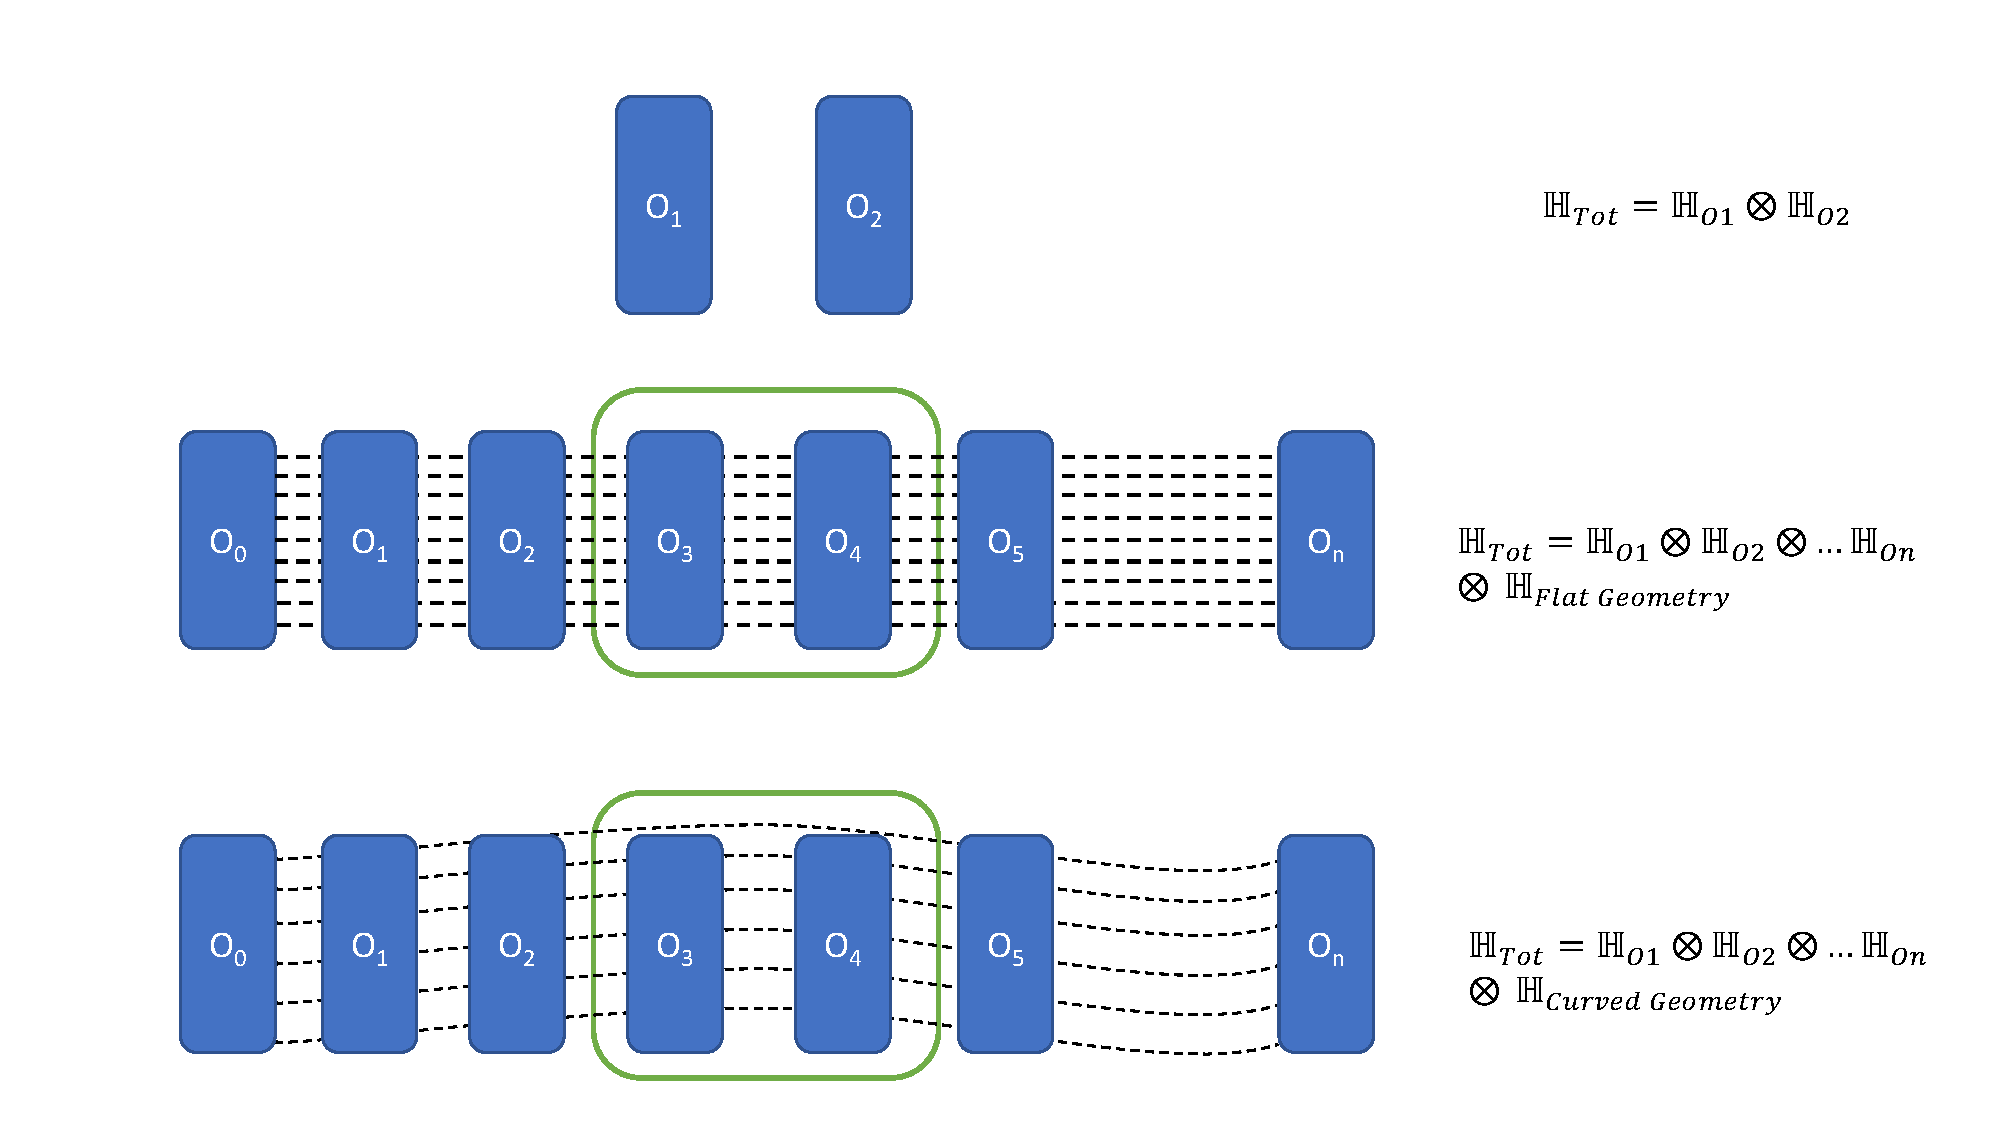
\includegraphics[width=\textwidth,height=10cm]{Schematic_oscillators.pdf}
\caption{Schematic of the three systems we study for their entanglement properties. The top sketch of two harmonic oscillators $O_1$ and $O_2$. The combined Hilbert space of the two oscillators is denoted by $\mathbb{H}_{Tot}$ which is the tensor product of the individual Hilbert spaces $\mathbb{H}_{O1}$ and $\mathbb{H}_{O2}$.The middle is a representative of a scalar quantum field that can be thought of as a collection of Harmonic oscillators. The total Hilbert space in this case is a tensor product of the individual harmonic oscillator Hilbert spaces and the Hilbert space of flat Minkowski space $\mathbb{H}_{Flat \ Geometry}$. The dotted lines represent the background spacetime - in this case flat space. The bottom sketch is a generalization of middle sketch as it contains the Hilbert space of a curved spacetime, $\mathbb{H}_{Curved \ Geometry}$.}
\label{osc}
\end{center}
\end{figure}

\begin{itemize}

\item A review of harmonic oscillators interacting via a perturbed Hamiltonian. 
In particular a Hamiltonian is constructed that is a sum of two Harmonic oscillators which interact via a perturbative interaction term.

\item Relationship between a discretized scalar field theory in flat space and a collection of harmonic oscillators. 
Inherent coupling of the harmonic oscillators (represented by the momentum modes) in a quantum field and the resulting entanglement. 
We make a comparison of this to the harmonic oscillator case by considering two momentum modes.


\item A generalization of the scalar field theory to curved space and a potential enhancement to entanglement due to curvature. 
We use to momenta modes of the scalar field coupled to a graviton mode from the background geometry. 

\end{itemize}

The paper is structured as follows. 
In section \ref{sec:QM} we review the quantum mechanical calculation of two free harmonic oscillators coupled through a quartic interaction. 
In section \ref{sec:QFTflat} a discretized free scalar field theory is constructed in terms of individual harmonic oscillators. 
In particular the momentum modes of the scalar field act as harmonic oscillators. 
The entanglement entropy and the evolution of the purity of the initial state is analyzed for the momentum modes. 
We also point out the difference in the entanglement structure in real space and momentum space for the quantum field. 
Section \ref{sec:QFTcurved} contains the generalization of free scalar fields in a curved spacetime. 
We analyze the same entanglement structure and compare it to the flat spacetime case. 
In particular we look for additional entanglement cause by entanglement between the scalar field momentum modes and the graviton modes. 
Finally in section \ref{sec:Discuss} we make some comments on the applications of results with a particular focus on the loss of unitarity in QFT's \cite{isheng1}. 
We also show how this might also hint to a solution to the black hole information problem as outlined in \cite{Baker:2017sgx}.

\section{Simple harmonic oscillator} \label{sec:QM}

We will study the system of two harmonic oscillators, governed by the Hamiltonian
\begin{align}
H_{AB} &= \frac{p^2_{1}}{2m} + \frac{p^2_{2}}{2m} + \frac{1}{2}m\omega_A^2x_A^2 + \frac{1}{2}m\omega_B^2x_B^2 + \frac{\alpha}{4} x_A^2x_B^2, \label{hamiltonian}
\\ &\equiv H_A + H_A + \Delta H_{AB}
\end{align}
coupled by some small parameter $\alpha \ll m^2\omega_A^2\omega_B^2$. In the case $\alpha = 0$ the oscillators are uncoupled and the ground state is the product state. First, we would like to perturb the two oscillator system with an $\alpha \neq 0$ and find the perturbed eigenstates. We would then like to expand the product (false) ground state in terms of the perturbed eigenfunctions,
\begin{align}
| 0^{(0)} 0^{(0)} \rangle = \sum_{k_1, k_2} \langle k_1 k_2 | 0^{(0)} 0^{(0)}\rangle | k_1 k_2 \rangle. \label{expand1}
\end{align} 
So we simply need to invert the standard perturbation expansion. The task of computing the non-zero perturbation matrix elements is greatly simplified by the property of the simple harmonic oscillator (SHO) that
\begin{equation}
\langle 0 | x^2 | k \rangle = c_1 \delta_{0k} + c_2 \delta_{2k},
\end{equation}
with $c_1 = \hbar / 2m\omega$ and $c_2 = \hbar \sqrt{2} / 2m\omega$. The only non-zero matrix elements are then
\begin{align}
V_{0000} &= \left( \frac{\hbar}{2m\omega_A}\right) \left( \frac{\alpha}{4}\right) \left( \frac{\hbar}{2m\omega_B}\right),
\\ V_{0020} &= \left( \frac{\hbar\sqrt{2}}{2m\omega_A}\right) \left( \frac{\alpha}{4}\right) \left( \frac{\hbar}{2m\omega_B}\right), 
\\ V_{0002} &= \left( \frac{\hbar}{2m\omega_A}\right) \left( \frac{\alpha}{4}\right) \left( \frac{\hbar\sqrt{2}}{2m\omega_B}\right), 
\\ {\rm and~} V_{0022} &= \left( \frac{\hbar\sqrt{2}}{2m\omega_A}\right) \left( \frac{\alpha}{4}\right) \left( \frac{\hbar\sqrt{2}}{2m\omega_B}\right).
\end{align}
Therefore Eq. (\ref{expand1}) becomes
\begin{align}
| 0^{(0)} 0^{(0)} \rangle &= \langle 00 | 0^{(0)} 0^{(0)}\rangle | 00 \rangle + \langle 02 | 0^{(0)} 0^{(0)}\rangle | 02 \rangle + \langle 20 | 0^{(0)} 0^{(0)}\rangle | 20 \rangle + \langle 22 | 0^{(0)} 0^{(0)}\rangle | 22 \rangle, \nonumber
\\ 
&= | 00 \rangle + \frac{V_{0002}}{E^{(0)}_{02} - E^{(0)}_{00}} | 02 \rangle + \frac{V_{0020}}{E^{(0)}_{20} - E^{(0)}_{00}}  | 20 \rangle + \frac{V_{0022}}{E^{(0)}_{22} - E^{(0)}_{00}} | 22 \rangle.
\label{expand2}
\end{align}
Having expanded the product ground state, the next step is to evolve this state with the time evolution operator and see that modes evolve which can not be expressed as a product (of the unperturbed eigenfunctions). To do this we should compute the density matrix and perform a partial trace over one of the individual oscillator states, then compute its entropy which should be non-zero. However, we are interested in computing the entropy of the evolved unperturbed ground state in the \textit{unperturbed} basis. Therefore we should evolve Eq. (\ref{expand2}) using the perturbed Hamiltonian, 
\begin{align}
U | 0^{(0)} 0^{(0)} \rangle = \sum_{k_1, k_2} \langle k_1 k_2 | 0^{(0)} 0^{(0)}\rangle e^{i(E_{k_1k_2})t/\hbar} | k_1 k_2 \rangle, \label{evolve1}
\end{align} 
then expand the result in the unperturbed basis.

The first thing we encounter when inspecting the expansion of the states $|k_1k_2\rangle$ is that the second excited states may superpose with the the fourth state. However, these terms all appear at $\mathcal{O}(\alpha^2)$ in the expansion of the evolved ground state, so we do not include them. To first order in $\alpha$, Eq. (\ref{evolve1}) becomes
\begin{align}
U | 0^{(0)} 0^{(0)} \rangle =~& e^{iE_{00}t/\hbar}\left( | 0^{(0)} 0^{(0)} \rangle +  C_{0200}| 0^{(0)} 2^{(0)} \rangle +  C_{2000}| 2^{(0)} 0^{(0)} \rangle +   C_{2200}| 2^{(0)} 2^{(0)} \rangle \right) \nonumber
\\ &+ C_{0002} e^{iE_{02}t/\hbar} | 0^{(0)} 2^{(0)} \rangle + C_{0020} e^{iE_{20}t/\hbar} | 2^{(0)} 0^{(0)} \rangle + C_{0022} e^{iE_{22}t/\hbar} | 2^{(0)} 2^{(0)} \rangle,
\end{align}
where the $C$s are the $V$s over the energies and so have the property that $C_{m_1m_2n_1n_2} = -C_{n_1n_2m_1m_2}$. Collecting terms,
\begin{align}
U | 0^{(0)} 0^{(0)} \rangle =&~| 0^{(0)} 0^{(0)} \rangle e^{iE_{00}t/\hbar}
\nonumber \\&+ | 0^{(0)} 2^{(0)} \rangle \left( C_{0002} e^{iE_{02}t/\hbar} + C_{0200} e^{iE_{00}t/\hbar}  \right)
\nonumber \\&+ | 2^{(0)} 0^{(0)} \rangle \left( C_{0020} e^{iE_{20}t/\hbar} + C_{2000} e^{iE_{00}t/\hbar} \right)
\nonumber \\&+ | 2^{(0)} 2^{(0)} \rangle \left( C_{0022} e^{iE_{22}t/\hbar} + C_{2200} e^{iE_{00}t/\hbar}\right). \label{evolved}
\end{align}
Before constructing the density we take note that the state Eq. (\ref{evolved}) is not properly normalized. These are $\mathcal{O}(\alpha^2)$ terms and so naively we should neglect them. However, since our goal is to evaluate the entropy of the reduced density matrix, we realize that $\mathcal{O}(\alpha^2)$ terms along the diagonal contribute at the same order as $\mathcal{O}(\alpha)$ terms on the off-diagonal to the eigenvalues. The only normalization term which contributes at this order sits in the $| 0^{(0)} 0^{(0)} \rangle \langle 0^{(0)} 0^{(0)} |$ element of the density matrix. To find the normalization $Z_{00}$, we use orthonormality of the normalized states to find
\begin{align}
\frac{1}{Z_{00}^2} &= 1 + \left( C_{0002} e^{i(E_{02}-E_{00})t/\hbar} + C_{0200} \right)^2
+ \left( C_{0020} e^{i(E_{20}-E_{00})t/\hbar} + C_{2000} \right)^2
+ \left( C_{0022} e^{i(E_{22}-E_{00})t/\hbar} + C_{2200} \right)^2, \label{normalization}
\\ \nonumber &\equiv 1 + D_{02}^2 + D_{20}^2 + D_{22}^2,
\end{align}
where for ease of notation in the following we have defined the $D$ parameters, which are complex and functions of time. We can now construct the density
\begin{align}
\rho_{AB} &= \sum_{m_1m_2,n_1n_2} | m_1^{(0)} m_2^{(0)} \rangle \langle m_1^{(0)} m_2^{(0)} | U | 0^{(0)} 0^{(0)} \rangle \langle 0^{(0)} 0^{(0)} | U | n_1^{(0)} n_2^{(0)} \rangle \langle n_1^{(0)} n_2^{(0)} | \label{density1},
\end{align}
and evaluate the partial trace over the first SHO. To first order in $\alpha$, the reduced density operator is then,
\begin{align}
\rho_{B} &= \sum_{k_1} \langle k_1 | \rho_{AB} | k_1 \rangle
\nonumber \\ & = 
\left( \begin{matrix}
 |  0^{(0)} \rangle \\
 |   2^{(0)} \rangle 
 \end{matrix} \right)
\left( \begin{matrix}
 Z_{00}^2 + D_{20}^2 & D_{02} \\
D_{02}^* & D_{02}^2 + D_{22}^2  \\
 \end{matrix} \right)
 \left( \begin{matrix}
  \langle 0^{(0)} | \\
  \langle  2^{(0)} |
 \end{matrix} \right),
 \nonumber \\ & = 
\left( \begin{matrix}
 |  0^{(0)} \rangle \\
 |   2^{(0)} \rangle 
 \end{matrix} \right)
\left( \begin{matrix}
 1 - D_{02}^2 - D_{22}^2 & D_{02} \\
D_{02}^* & D_{02}^2 + D_{22}^2  \\
 \end{matrix} \right)
 \left( \begin{matrix}
  \langle 0^{(0)} | \\
  \langle  2^{(0)} |
 \end{matrix} \right). \label{reduceddensity1}
\end{align}
As expected, due to the antisymmetry of the $C$ constants, all of the $D^2$ terms increase from $0$ at $t=0$, meaning reduced density matrix evolves from a trivial one at $t=0$. For $t\neq 0$ the system becomes entangled. We can see this explicitly by computing the entropy
\begin{equation}
S = \lambda_1 {\rm log} \lambda_1 + \lambda_2 {\rm log} \lambda_2,
\end{equation}
where the $\lambda_i$ are the eigenvalues of the reduced density matrix, given by
\begin{align}
\lambda_1 &= 1 - D_{22}^2 = 1 - 4C^2 \sin^2{((\omega_A + \omega_B)t)}, \label{eig1}
\\ \lambda_2 &= D_{22}^2 = 4C^2 \sin^2{((\omega_A + \omega_B)t)}, \label{eig2}
\end{align}
and 
\begin{align}
C^2 \equiv C_{0022}^2 =  C_{2200}^2 = \left(\frac{\left( \frac{\hbar\sqrt{2}}{2m\omega_A}\right) \left( \frac{\alpha}{4}\right) \left( \frac{\hbar\sqrt{2}}{2m\omega_B}\right)}{2\hbar (\omega_A + \omega_B)}\right)^2. \label{constant}
\end{align}
Note that for $\alpha = m^2 \omega_A^2\omega_B^2$, the case in which the perturbation is just the product of the unperturbed potentials, Eq. (\ref{constant}) becomes $C^2 =  \left( \frac{\hbar \omega_A\omega_B}{4(\omega_A + \omega_B)} \right)^2$. 

%%%%%%%%%%%%%%%%%%%%%%%%%%
\section{Discretized quantum field thoery} \label{sec:QFTflat}

\subsection{Formalism of discretization of free fields in momentum space}

We work in the Schrodinger picture, thus the fields will be time-independent, $\phi(\vec{x})$. 
The Hamiltonian of a free scalar field is

\begin{equation}
	H = \int d^3x \left( \frac{1}{2} \pi^2(\vec{x}) + \frac{1}{2} (\nabla \phi(\vec{x}))^2 + \frac{1}{2} m^2 \phi^2(\vec{x}) \right)	\label{free-scalar hamiltonian}
\end{equation}

where $\pi(\vec{x})$ is the conjugate momentum of $\phi(\vec{x})$. 
To make contact with the quantum mechanics we want to discretize the modes of these fields. 
The first step is to discretize the 3 space dimensions $\vec{x}$.
Lets do this by restricting the space to be a box of size $L^3$. 
It is also useful to define periodic boundary conditions, this is useful when we expand the fields in Fourier modes as it will tell us which functions are good for expanding. 
The boundary conditions are of the form $\phi(\vec{x}) = \phi(\vec{x}  + L)$. 
This gives discrete plane wave modes. 

\begin{equation}
	\psi_{\vec{k}}(\vec{x}) = L^{-\frac{3}{2}} e^{i \vec{k} \vec{x}}
\end{equation}

where $k_x,k_y,k_z = \frac{2 \pi n}{L}$ where $n$ is an integer. 
The scalar field can now be expanded in terms of these functions. 

\begin{eqnarray}
	\phi(\vec{x}) & = & \sum_{\vec{k}} \ L^{-\frac{3}{2}} e^{i \vec{k} \vec{x}} \ \phi_{\vec{k}}	\nonumber	\\
	\pi(\vec{x}) & = & \sum_{\vec{k}} \ L^{-\frac{3}{2}} e^{i \vec{k} \vec{x}} \ \pi_{\vec{k}}	\nonumber	\\
	\phi_{\vec{k}} & = & \int^{\vec{L}/2}_{-\vec{L}/2} d^3 \vec{x} \ L^{-\frac{3}{2}} e^{-i \vec{k} \vec{x}} \ \phi(\vec{x})	\nonumber	\\
	 \pi_{\vec{k}} & = & \int^{\vec{L}/2}_{-\vec{L}/2} \ d^3 \vec{x} \ L^{-\frac{3}{2}} e^{-i \vec{k} \vec{x}} \ \pi(\vec{x})
\end{eqnarray}
	
The commutation relation between these fields are 

\begin{eqnarray}
	& & [\phi_{\vec{k}'}, \phi_{\vec{k}}] = 0	\nonumber	\\
	& & [\pi_{\vec{k}}, \pi_{\vec{k}'} ] = 0	\nonumber	\\
	& & [\vec{\phi}_{\vec{k}}, \pi_{\vec{k}'}] = \int^{\vec{L}/2}_{-\vec{L}/2} d^3 \vec{x}\int^{\vec{L}/2}_{-\vec{L}/2} d^3 \vec{x'} \ L^{-3} e^{-i \vec{k} \vec{x}} e^{-i \vec{k}' \vec{x}'} \ [\phi(\vec{x}), \pi(\vec{x}')]	\nonumber	\\
	& & = i L^{-3} \int^{\vec{L}/2}_{-\vec{L}/2} \ d^3 \vec{x} e^{-i\vec{x}(\vec{k} + \vec{k}')} = i \delta_{\vec{k},-\vec{k}'} 
\end{eqnarray}

We note that the mode operators $\phi_{\vec{k}}$, $\pi_{\vec{k}}$ are not Hermitian. 

\begin{equation}
	\phi^\dagger_{\vec{k}} = \phi_{- \vec{k}}, \ \ \ \pi^\dagger_{\vec{k}} = \pi_{- \vec{k}}
\end{equation}

Using this we can write the following commutation relations

\begin{eqnarray}
	& & [\phi_{\vec{k}}, \pi^\dagger_{\vec{k}'} ] = [\phi^\dagger_{\vec{k}}, \pi_{\vec{k}'}] = i \delta_{\vec{k}, \vec{k}'}	\nonumber	\\
	 & &  [\phi_{\vec{k}}, \pi_{\vec{k}'} ] = [\phi^\dagger_{\vec{k}}, \pi^\dagger_{\vec{k}'}] = i \delta_{\vec{k} + \vec{k}', 0}
\end{eqnarray}

Now we can write the Hamiltonian in terms of these modes. Lets compute the required ingredients first

\begin{eqnarray}
	\int \ d^3 \vec{x} \ \pi^2(\vec{x}) & = & \int \ d^3 \vec{x} \pi^\dagger(\vec{x}) \pi(\vec{x}) = \int d^3 \vec{x} \sum_{\vec{k}} \sum_{\vec{k}'} L^{-3} e^{-i \vec{k} \vec{x}} e^{i\vec{k}' \vec{x}} \ \pi^\dagger_{\vec{k}} \pi^\dagger_{\vec{k}} \pi_{\vec{k}'}	\nonumber	\\
	& = & \sum_{\vec{k}, \vec{k}'} \pi^\dagger_{\vec{k}} \pi_{\vec{k}'} \ \left( L^{-3} \int^{\vec{L}/2}_{-\vec{L}/2} d^3 \vec{x} e^{i \vec{x}(\vec{k}' - \vec{k})} \right)	\nonumber	\\
	& = & \sum_{\vec{k}} \pi^\dagger_{\vec{k}} \pi_{\vec{k}}
\end{eqnarray} 

Similarly we get

\begin{equation}
	\int d^3 \vec{x} \phi^2 (\vec{x}) = \sum_{\vec{k}} \phi^\dagger_{\vec{k}} \phi_{\vec{k}}
\end{equation}

We can expand the gradient term as

\begin{equation}
	\nabla \phi_{\vec{x}} = \sum_{\vec{k}} L^{-\frac{3}{2}} e^{i \vec{k} \vec{x}} \ i \vec{k} \phi_{\vec{k}} = -i \sum_{\vec{k}}L^{-\frac{3}{2}} e^{-i \vec{k} \vec{x}} \vec{k} \phi^\dagger_{\vec{k}}
\end{equation}

\begin{equation}	
	\int \ d^3 \vec{x} ( \nabla \phi(\vec{x}))^2 = \sum_{\vec{k}} \ \vec{k}^2 \ \phi^\dagger_{\vec{k}} \phi_{\vec{k}}
\end{equation}

This gives the Hamiltonian

\begin{equation}
	H = \sum_{\vec{k}} \left( \frac{1}{2} \pi^\dagger_{\vec{k}} \pi_{\vec{k}} + \frac{1}{2} (\vec{k}^2 + m^2) \phi^\dagger_{\vec{k}} \phi_{\vec{k}} \right)
\end{equation}

It is apparent that this Hamiltonian represents that of a collection of harmonic oscillators with frequencies $\omega_{\vec{k}} = \sqrt{\vec{k}^2 + m^2}$. 
The mode operators are not Hermitian and so we need to be careful into getting the mode operators in terms of the ladder operators. 
We define

\begin{eqnarray}
	a_{\vec{k}} & = & \frac{1}{\sqrt{2 \omega_{\vec{k}}}} \left( \omega_{\vec{k}} \phi_{\vec{k}} + i \pi_{\vec{k}} \right) \nonumber	\\
	a^\dagger_{\vec{k}} & = & \frac{1}{\sqrt{2 \omega_{\vec{k}}}} \left( \omega_{\vec{k}} \phi^\dagger_{\vec{k}} - i \pi^\dagger_{\vec{k}} \right)	\nonumber	\\
	a_{- \vec{k}} & = & \frac{1}{\sqrt{2 \omega_{\vec{k}}}} \left( \omega_{\vec{k}} \phi^\dagger_{\vec{k}} + i \pi^\dagger_{\vec{k}} \right)	\nonumber	\\
	a^\dagger_{- \vec{k}} & = & \frac{1}{\sqrt{2 \omega_{\vec{k}}}} \left( \omega_{\vec{k}} \phi_{\vec{k}} - i \pi_{\vec{k}} \right)
\end{eqnarray}

These have the following commutation relations

\begin{eqnarray}
	[a_{\vec{k}}, a_{\vec{k}'}] & = & \frac{1}{\sqrt{4 \omega \omega'}} \left( \omega \omega' [\phi_{\vec{k}}, \phi_{\vec{k}'}] + i \omega' [\pi_{\vec{k}}, \phi_{\vec{k}'}] + i \omega[\phi_{\vec{k}}, \phi_{\vec{k}'}] - [\pi_{\vec{k}}, \pi_{\vec{k}'}] \right)	\nonumber	\\
	& = & \frac{1}{\sqrt{4 \omega \omega'}} (0 + i \omega' (- i \delta_{\vec{k} + \vec{k}',0}) + i\omega(i \delta_{\vec{k} + \vec{k}',0}) + 0)	\nonumber	\\
	& = & \delta_{\vec{k} + \vec{k}',0} \left( \frac{\omega' - \omega}{\sqrt{4 \omega \omega'}} \right)	= 0
\end{eqnarray}

because $\vec{k} = - \vec{k}'$ means $\omega' = \omega$. 

The other commutation relations are

\begin{equation}
	[a_{\vec{k}}, a^\dagger_{\vec{k}'}] = \delta_{\vec{k}, \vec{k}'}
\end{equation}

\begin{equation}
	[a^\dagger_{\vec{k}}, a^\dagger_{\vec{k}'}] = 0
\end{equation}

Adding and subtracting these equations we find

\begin{equation}
	a^\dagger_{- \vec{k}} + a_{\vec{k}} = \sqrt{2 \omega_{\vec{k}}} \phi_{\vec{k}}
\end{equation}

\begin{equation}
	-ia_{\vec{k}} + i a^\dagger_{- \vec{k}} = \sqrt{\frac{2}{\omega_{\vec{k}}}} \pi_{\vec{k}}
\end{equation}

Using this we can write the Hamiltonian in terms of the ladder operators

\begin{equation}
	H = \sum_{\vec{k}} \omega_{\vec{k}} \left( a^\dagger_{\vec{k}} a_{\vec{k}} + \frac{1}{2} \right)
\end{equation}

This is the Hamiltonian for many harmonic oscillators. 

%%%%%%%%%%%%%%%%%%%%%
\subsection{Real space discretization}

We know attempt to discretize the Hamiltonian in Eq (\ref{free-scalar hamiltonian}) this in real space immediately. 

\begin{equation}
	H_{free} = \vec{l}^3 \sum_{\vec{n}}^{\vec{L}/\vec{l}} \ \frac{1}{2} \left( \dot{\phi}^2_{\vec{n}} + \vec{l}^{-2} ( \phi_{\vec{n} + 1} - \phi_{\vec{n}})^2 \right)
\end{equation}

Here we use vector notation to denote the fact that we are discretizing three dimensions.
Next we consider two modes of the quantum fields "localized'' at positions $A$ and $B$. 
In this case the Hamiltonian becomes

\begin{equation}
	H_{free} = \frac{1}{2} l^3 \left( \dot{\phi}^2_B + \dot{\phi}^2_A + l^{-2} (\phi_B - \phi_A)^2 \right)
\end{equation}

Thus we see that the spatial gradient term will couple the two modes, even in free field theory. We can thus redefine these fields as

\begin{equation}
	\phi_A = \phi_+ + \phi_-, \ \phi_B = \phi_+ - \phi_-
\end{equation}

The Hamiltonian in terms of the new fields $\phi_+$ and $\phi_-$ is

\begin{equation}
	H_{free} = \frac{l^3}{2} \left( \dot{\phi}_+^2 + \dot{\phi}_-^2 + \frac{4 \phi_-^2}{l^2} \right)
\end{equation}

We can write the $\phi_+$ and $\phi_-$ can be written in terms of ladder operators

\begin{eqnarray}
	\phi_+ & = & \phi_{p+} (a+a^\dagger)	\nonumber	\\
	\phi_- & = & \phi_{p-}(b+b^\dagger)
\end{eqnarray}

where $\phi_{p_-}$, $\phi_{p+}$ are some normalizations that depend on the momenta. The free Hamiltonian can be written as

\begin{eqnarray}
	H_{free} & = & H_{HO} + H_{QFT/HO}	\nonumber	\\
	H_{HO} & = & \dot{\phi}^2_{p+} \left( a^\dagger a + \frac{1}{2} \right) + \dot{\phi}^2_{p-} \left( b^\dagger b + \frac{1}{2} \right)	\nonumber	\\
	H_{QFT/HO} & = & \dot{\phi}^2 _{p+} \left(a^2 + {a^\dagger}^2 \right) + \dot{\phi}^2_{p-} \left(b^2 + {b^\dagger}^2 \right) + \frac{1}{2} \frac{\phi_{p-}}{l^2} \left( b^2 + {b^\dagger}^2 \right) + \frac{1}{2} \frac{\phi^2_{p-}}{l^2} \left( b^\dagger b + \frac{1}{2} \right) 
\end{eqnarray}

We see that the first term is the same as two free harmonic oscillators. 
The second term is a correction coming from field theory. 
We can compute the correction to the vacuum state of the free field theory by the additional operators in the $H_{QFT/HO}$ Hamiltonian. 
We use the formalism of Time Independent Perturbation Theory (TIPT). The first order correction to a known state $|\psi_1 \rangle$ due to a perturbative Hamiltonian is given by

\begin{equation}
	|\psi_1 \rangle  = \sum_{m_1, m_2 \neq i_1,i_2} \frac{\langle i^{(1)} i^{(2)}|H_{per}|m^{(1)} m^{(2)} \rangle}{E^{(0)}_{i^1i^2} - E^{(0)}_{m^1m^2}} |m^{(1)}m^{(2)} \rangle 
\end{equation}

here $H_{per}$ is a perturbative Hamiltonian. $|i^{(1)} i^{(2)}\rangle$ is the initial state of the system. 
The superscript is there to represent the particle being referred to (we have only put two particles here since that is the system we are considering but in general it could be any number of particles). 
The energies $E^{(0)}_{i^1i^2}$ represents the unperturbed energy of the system in its initial state and similarly the energy for the $m^1m^2$ state is defined. 
Note that these states are in the Hilbert space of the \underline{unperturbed} Hamiltonian. 
Using this we can use $H_{QFT/HO}$ as a perturbative Hamiltonian and the initial state to be a vacuum state to get 

\begin{equation}
	|\psi_1 \rangle = |00 \rangle + \frac{\sqrt{2} \dot{\phi}^2_{p+}}{E^{(0)}_{00} - E^{(0)}_{20}} |20 \rangle + \left( \frac{\sqrt{2} \dot{\phi}^2_{p-}}{E^{(0)}_{00} - E^{(0)}_{02}} + \frac{4 \phi_{p-}}{\sqrt{2} l^2(E^{(0)}_{00} - E^{(0)}_{02})} \right) | 02 \rangle
\end{equation}

We can apply the time evolution operator to get

\begin{eqnarray}
	|\psi_1(t) \rangle & = & e^{-iH_{HO}t}(|\psi_0 \rangle + | \psi_1 \rangle) = e^{-iE_{00}^{(0)}t} |00 \rangle + e^{-iE_{02}t} \left( \frac{\sqrt{2} \dot{\phi}^2_{p+}}{E^{(0)}_{00} - E^{(0)}_{20}} |20 \rangle + \left( \frac{\sqrt{2} \dot{\phi}^2_{p-}}{E^{(0)}_{00} - E^{(0)}_{02}} + \frac{4 \phi_{p-}}{\sqrt{2} l^2(E^{(0)}_{00} - E^{(0)}_{02})} \right) | 02 \rangle \right)	\nonumber	\\
	& \equiv & c_{00} | 00 \rangle + c_{20} |20 \rangle + c_{02} |02 \rangle
\end{eqnarray}
	
where we have made use of the fact that $E_{02} = E_{20}$ and that $|\psi_0 \rangle = |00\rangle$. The density matrix can now be written down as

\begin{equation}
	\rho = |\psi(t) \rangle \langle \psi(t)| = \begin{pmatrix} |c_{00}|^2 & c_{00} c^*_{20} & c_{00} c^*_{02} \\
	c_{00}c^*_{20} & |c_{20}|^2 & c_{20} c^*_{02} \\
	c_{00}c_{02}^* & c_{20} c^*_{02} & |c_{02}|^2 \end{pmatrix}
\end{equation}

The partial trace over the second system, $A$ will give the reduced density matrix for $B$

\begin{equation}
	\rho_B = tr_A \rho = \begin{pmatrix} 1 + |c_{20}|^2 & c^*_{02} \\ c_{02} & |c_{02}|^2 \end{pmatrix}
\end{equation}




%%%%%%%
\subsection{$\phi^4$ case}
Here we will discuss the analogy between the coupled harmonic oscillators and a self interacting scalar quantum field theory with Hamiltonian

\begin{equation}
H = \int d^3x~ \left( \frac{1}{2} \pi^2 + \frac{1}{2} (\nabla \phi)^2 + \frac{1}{2}m^2\phi^2 + \frac{\lambda^4}{4}\phi^4\right).
\end{equation}
In the case $\lambda = 0$, the theory corresponds to a free scalar field which follows the Klein-Gordon equations of motion. The solutions to this equation are the Fourier modes of the classical scalar field, which are as a result uncoupled in the Hamiltonian and evolve independently. Imposing canonical equal-time commutation relations
\begin{equation}
[\pi(x, t), \phi(y, t)] = i \delta^3(x - y),
\end{equation}
we can identify the positive and negative modes with the creation and annihilation operators of an infinite set of uncoupled harmonic oscillators. However, for $\lambda \neq 0$ these modes will generally be coupled. We would like to study the evolution of entanglement between any two of these modes. 

\subsection{Two state case} \label{subsec:twostate}

To do so, we at first introduce the heavy simplifications of a finite box size $L$ and a lattice spacing $\Delta x$. Further, we choose a theory which contains only two space-time points $x_1$ and $x_2$, so that $L = 2 \Delta x$. In this theory therefore, there are only two possible modes. From the mode expansion
\begin{equation}
\phi(x_m) = \frac{1}{N} \sum_{n = 0}^{N - 1} (\tilde{\phi}(k_n) e^{i \frac{2\pi}{N} m n} + \tilde{\phi}^*(k_n)  e^{-i \frac{2\pi}{N} m n}), 
\end{equation}
where $N = L/\Delta x$ is the number of modes, for $N=2$ we see that,
\begin{align}
\phi(x_1) &= \frac{1}{2} (\phi^+ + \phi^-), 
\\ {\rm and} ~~\phi(x_2) &= \frac{1}{2} (\phi^+ - \phi^-), 
\end{align}
where we have defined $\phi^+ \equiv (\tilde{\phi}(k_0) + \tilde{\phi}^*(k_0))$ and $\phi^- \equiv (\tilde{\phi}(k_1) + \tilde{\phi}^*(k_1))$, which represent the sum and difference of the spatial field values (essentially all the information we could have about the field). 

For the quantized theory $\phi^+$ and $\phi^-$ represent the sum of the lowering and raising operators of their corresponding mode and are therefore equivalent to the position operators of quantum mechanics. We can verify that $\phi^+$ and $\phi^-$ are uncoupled in the free field Hamiltonian and that they commute. Expanding the coupling term of the Hamiltonian
\begin{align}
\frac{\lambda^4}{4}\left(\phi(x_1)^4 + \phi(x_2)^4 \right)= \frac{\lambda^4}{4} \frac{1}{2^4}\left(  2 \phi^{+^{4}} + 12 \phi^{+^{2}}\phi^{-^{2}} + 2 \phi^{-^{4}}\right).
\end{align}
All odd terms cancel in the sum over space and the resulting coupling is almost identical to the QHO case, except for an extra $\phi^4$ self-coupling. Naively we might worry that these terms could have some non-linear effect on the development of entanglement (i.e. that we must modify Section \ref{sec:warmup}), since a coupling between the ground and the 4th excited single-oscillator state is introduced at the same order in perturbation theory we have been considering. However, inspecting the eigenvalues Eqs. \eqref{eig1} and \eqref{eig2} we recall that for the quadratic coupling entanglement was controlled only by the $D_{22}$ parameter. We see that the $\phi^4$ terms do not contribute to the entanglement (except through their shifts in the energies) since $D_{44}$ is zero, as expected since they introduce no coupling between modes.

\subsection{A one-dimensional chain} \label{subsec:1d}

For a full one-dimensional chain, to determine the coupling in the Hamiltonian, we must evalute the sum

\begin{align}
\frac{\lambda^4}{4}\sum_m \phi(x_m)^4 =
\frac{\lambda^4}{4} \sum_m \left( \frac{1}{N} \sum_{n}^{N - 1} (\tilde{\phi}(k_n) e^{i \frac{2\pi}{N} m n} + \tilde{\phi}^*(k_n)  e^{-i \frac{2\pi}{N} m n})\right)^4
\end{align}

There will be only certain (7) kinds of terms that can arise to couple to any one mode $n^*$.
\begin{align*}
& n^* = n' = n'' = n''' ~(\phi^4 {\rm ~term}), \\
& n^* = n' \neq n'' = n''' ~(\phi^2\phi^2 {\rm ~term}), \\
& n^* \neq n' \neq n'' \neq n''' ~(\text{a coupling to 3 other modes}), \\
& n^* \neq n' = n'' = n''', ~(\phi\phi^3 {\rm ~term}),\\
& n^* = n' = n'' \neq n''',  ~(\phi^3\phi {\rm ~term}),\\
& n^* = n' \neq n'', n''',  ~(\phi^2\phi\phi {\rm ~term}),\\
& n^*, n' \neq n'' = n''', ~(\phi\phi\phi^2 {\rm ~term}).
\end{align*}

%%%%%%%%
\section{Discretized scalar fields in curved space} \label{sec:QFTcurved}

%%%%%%%%
\section{Discussion} \label{sec:Discuss}


\bibliography{entanglementbib}


%%%%%%%%%%%%%%%%%%%%%%%%%%%%%%%%%%%%%%%%%%%%%%%%%%%%%%%%%%%%%%%%%%%%%%%%
\end{document}
